\chapter{Data Validation Testing}

	The most common web application security weakness is the failure to properly validate input coming 
	from the client or environment before using it.  Data validation is the task of testing all the 
	possible forms of input, to understand if the application sufficiently validates input data before 
	using it.

\section{Cross Site Scripting (XSS)}

	In Cross Site Scripting (XSS) testing, we test if it is possible to manipulate the input parameters 
	of the application so that it generates malicious output. We find an XSS vulnerability when the
	application does not validate our input and creates an output that is under our control. 

	\subsection{Refelcted Cross Site Scripting}
		Reflected XSS attacks are also known as {\bf type 1 or non-persistent XSS} attacks, and are 
		the most frequent type of XSS attacks found nowadays.
		When a web application is vulnerable to this type of attack, it will pass unvalidated input 
		sent through requests to the client. The common modus operandi of the attack includes a design 
		step, in which the attacker creates and tests an offending URI, a social engineering step, 
		in which she convinces her victims to load this URI on their browsers, and the eventual execution 
		of the offending code — using the victim's credentials.

		One of the important matters about exploiting XSS vulnerabilities is {\bf character encoding}. 
		In some cases, the web server or the web application could not be filtering some encodings of
		characters, so, for example, the web application might filter out a script tag, but might not 
		filter \%3cscript\%3e which simply includes another encoding of tags. 

		{\bf Example:}

		consider a site that has a welcome notice " Welcome \%username\% " and a download link.


		\begin{figure}[H]
			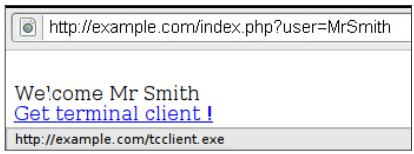
\includegraphics[scale=0.5]{pics/xxs1.png}
		\end{figure}

		To analyze it, the tester will play with the user variable and try to trigger the vulnerability. 
		Let's try to click on the following link and see what happens: 

		\begin{figure}[H]
			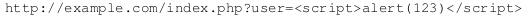
\includegraphics[scale=0.5]{pics/link.png}
		\end{figure}
		If no sanitization is applied this will result in the following popup:

		\begin{figure}[H]
			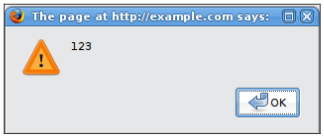
\includegraphics[scale=0.5]{pics/xss2.png}
		\end{figure}

		This indicates that there is an XSS vulnerability and it appears that the tester can execute 
		code of his choice in anybody's browser if he clicks on the tester's link.

	\clearpage
	\subsection{Stored Cross Site Scripting}

		Stored Cross Site Scripting (XSS) is the most dangerous type of Cross Site Scripting. 
		Web applications that allow users to store data are potentially exposed to this type of 
		attack. Stored XSS occurs when a web application gathers input from a user which might 
		be malicious, and then stores that input in a data store for later use. The input that 
		is stored is not correctly filtered. As a consequence, the malicious data will appear
		to be part of the web site and run within the user’s browser under the privileges of the 
		web application. Stored XSS does not need a malicious link to be exploited. 
		A successful exploitation occurs when a user visits a page with a stored XSS.

		The first step is to identify all points where user input is stored into the back-end and 
		then displayed by the application. Typical examples of stored user input can be found in:
		User/Profiles page, shopping cart, file managers, application settings/preferences, etc.

		{\bf Example: }

		\begin{figure}[H]
			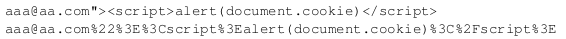
\includegraphics[scale=0.5]{pics/link2.png}
		\end{figure}
		\begin{figure}[H]
			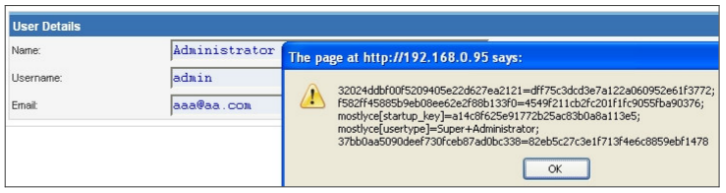
\includegraphics[scale=0.5]{pics/xss3.png}
		\end{figure}

	\subsection{DOM based Cross Site Scripting}
		Not all XSS bugs require the attacker to control the content returned from the server, but 
		can rather abuse poor JavaScript coding practices to achieve the same results. 
		The results are the same as a typical XSS bug, only the means of delivery is different.
		In comparison to other cross site scripting vulnerabilities (reflected and stored XSS), 
		where an unsanitized parameter is passed by the server, returned to the user and executed 
		in the context of the user’s browser, a DOM based cross site scripting vulnerability controls 
		the flow of the code by using elements of the Document Object Model (DOM) along with code 
		crafted by the attacker to change the flow.

		An attacker may append \# \textless script\textgreater alert('xss')\textless /script\textgreater to the affected page URL which would, 
		when executed display the alert box. In this instance, the appended code would not be sent 
		to the server as everything after the \# character is not treated as part of the query by 
		the browser but yet as a fragment. In this example the code is immediately executed and an
		alert of "xss" is displayed in the page. Unlike the more common types of cross site scripting 
		(persistent and non-persistent), in which the code is sent to the server and redisplayed to 
		the user, this is immediately executed in the user’s browser.


	\subsection{Cross Site Flashing}
	**RELEVANT?**

\section{SQL Injections (SQLi)}
	A SQL injection attack consists of insertion or "injection" of a SQL query via the input data 
	from the client to the application. A successful SQL injection exploit can read sensitive data 
	from the database, modify database data (Insert/Update/Delete), execute administration operations 
	on the database (such as shutdown the DBMS), recover the content of a given file existing on 
	the DBMS file system and, in some cases, issue commands to the operating system. 

	SQL Injection attacks can be divided into the following three classes:
		\begin{itemize}
			\item {\bf Inband:} data is extracted using the same channel that is used to inject the 
			SQL code. This is the most straightforward kind of attack, in which the retrieved data 
			is presented directly in the application web page.
			\item {\bf Out-of-band:} data is retrieved using a different channel (e.g., an email with the 
			results of the query is generated and sent to the tester).
			\item {\bf Inferential:} there is no actual transfer of data, but the tester is able to
			reconstruct the information by sending particular requests and observing the resulting 
			behaviour of the DB Server.
			\item {\bf Blind: } if the application hides the error details, then the tester must be 
			able to reverse engineer the logic of the original query.
		\end{itemize}

	{\bf SQL Injection Detection} \\
	The first step in this test is to understand when our application connects to a DB Server in order 
	to access some data. Typical examples of cases when an application needs to talk to a DB include:
	Authentication forms, search engines, E-Commerce sites, etc.

	The very first test usually consists of adding a single {\bf quote (')} or a {\bf semicolon (;)} 
	to the field  under test. The first is used in SQL as a string terminator and, if not filtered by 
	the application, would lead to an incorrect query. The second is used to end a SQL statement and, 
	if it is not filtered, it is also likely to generate an error. 

	{\bf Union Query SQL Injection} \\
	Another test involves the use of the UNION operator. This operator is used in SQL injections to 
	join a query, purposely forged by the tester, to the original query. The result of the forged 
	query will be joined to the result of the original query, allowing the tester to obtain the 
	values of fields of other tables.

	{\bf Blind SQL Injection} \\
	We have pointed out that there is another category of SQL injection, called Blind SQL Injection, 
	in which nothing is known on the outcome of an operation. For example, this behavior happens in 
	cases where the programmer has created a custom error page that does not reveal anything on 
	the structure of the query or on the database. (The page does not return a SQL error, it may 
	just return a HTTP 500).

	{\bf Stored Procedure Injections}
	When using dynamic SQL within a stored procedure, the application must properly sanitize the user 
	input to eliminate the risk of code injection. If not sanitized, the user could enter malicious 
	SQL that will be executed within the stored procedure.


\section{XML Injection}
	We talk about XML Injection testing when we try to inject an XML doc to the application: if the 
	XML parser fails to make an appropriate data validation the test will results positive.
	After lookking at a application, the tester will have some information about XML structure, 
	so it will be possible to try to inject XML data and tags (Tag Injection).

	{\bf Discovery} \\
	The first step in order to test an application for the presence of a XML Injection vulnerability,
	consists of trying to insert XML metacharacters.
	A list of some XML metacharacters is:
	\begin{itemize}
		\item Single quote {\bf '}
		\item Double quote {\bf "}
		\item Angular pharenthesis {\bf < >}
		\item Comment tag {\bf <!-- / -->}
		\item Ampersand {\bf \&}
	\end{itemize}

\section{SSI Injection}
	Web servers usually give to the developer the possibility of adding small pieces of dynamic code 
	inside static HTML pages, without having to play with full-fledged server-side or client-side 
	languages. This feature is incarnated by the Server-Side Includes (SSI), a very simple extension 
	that can enable an attacker to inject code into HTML pages, or even perform remote
	code execution.

	Putting an SSI directive into a static HTML document is as easy as writing a piece of code like 
	to print out the current time or like to include the content of a file.
	We could guess if SSI are supported just looking at the content of the target web site we are testing: 
	if it makes use of {\bf .shtml} files then SSI are probably supported, as this extension is used to
	identify pages containing these directives.

\section{Buffer Overflow}

	\subsection{Heap Overflow}
		Heap is a memory segment that is used for storing dynamically allocated data and global 
		variables. Each chunk of memory in heap consists of boundary tags that contain memory 
		management information. When a heap-based buffer is overflown, the control information 
		in these tags is overwritten, and when the heap management routine frees the buffer, 
		a memory address overwrite take place leading to an access violation. 

	\subsection{Stack Overflow}
		Stack overflows occur when variable size data is copied into fixed length buffers located 
		on the program stack without any bounds checking. 
		The key to testing an application for stack overflow vulnerabilities is supplying overly 
		large input data as compared to what is expected. 
